\documentclass[12pt,letterpaper]{exam}
\usepackage[lmargin=1in,rmargin=1in,tmargin=1in,bmargin=1in]{geometry}
\usepackage{../style/exams}

% -------------------
% Course & Exam Information
% -------------------
\newcommand{\course}{MATH 142: Final Exam}
\newcommand{\term}{Fall --- 2025}
\newcommand{\examdate}{12/09/2025}
\newcommand{\timelimit}{150 Minutes}

\setbool{hideans}{false} % Student: True; Instructor: False

\newcommand{\boxseven}[4]{%
	\draw[thick] (0,0) -- (4,0) -- (4,4) -- (0,4) -- (0,0);
	\draw[thick] (0,2) -- (4,2);
	\draw[thick] (2,0) -- (2,4);
	% '7'
	\draw[line width=0.03cm] (1.7,2.2) -- (2.3,2.2) -- (1.7,1.6);
	% Entries
	\node at (1,3) {$#1$};	% u
	\node at (3,1) {$#2$};	% dv
	\node at (1,1) {$#3$};	% du
	\node at (3,3) {$#4$};	% v
}
\usetikzlibrary{calc}
\usepackage{booktabs}
\tikzset{Arrow Style/.style={text=black, font=\boldmath}}
\newcommand{\tikzmark}[1]{%
    \tikz[overlay, remember picture, baseline] \node (#1) {};%
}
\newcommand*{\XShift}{0.5em}
\newcommand*{\YShift}{0.5ex}
\NewDocumentCommand{\DrawArrow}{s O{} m m m}{%
    \begin{tikzpicture}[overlay,remember picture]
        \draw[->, thick, Arrow Style, #2] 
                ($(#3.west)+(\XShift,\YShift)$) -- 
                ($(#4.east)+(-\XShift,\YShift)$)
        node [midway,above] {#5};
    \end{tikzpicture}%
}

% -------------------
% Content
% -------------------
\begin{document}

\examtitle
\instructions{Write your name on the appropriate line on the exam cover sheet. This exam contains \numpages\ pages (including this cover page) and \numquestions\ questions. Check that you have every page of the exam. Answer the questions in the spaces provided. Be sure to follow instructions, answer every question completely, and show all your work.} 
\scores
\bottomline
\newpage

% Poem
\phantom{.} \vfill
	\begin{table}[h]
	\centering
	\begin{tabular}{l}
	{\itshape ’Twas the night before Christmas, all frozen and still,} \\
	{\itshape Santa is working hard, but Math makes him quite ill.} \\
	{\itshape The sleigh is loaded, and the reindeer are prepared,} \\ 
	{\itshape But with problems unsolved, no gifts can be shared.} \\
	\\
	{\itshape ``These problems are hard!'', Santa cried out in fright.} \\
	{\itshape ``It's clear all my derivatives and sums aren't right!''} \\
	{\itshape This math needs to be done before Santa can take flight,} \\
	{\itshape He'll need a Calculus ace to help Save Christmas tonight!}
	\end{tabular}
	\end{table}
\phantom{.} \vfill 

% -------------------
% Questions
% -------------------
\begin{questions}

% Question 1
\newpage
\question[10] {\itshape On the brink of his flight, Santa is overcome with dismay, \par\phantom{(XX.. point)} For he'd forgotten his integrals, quick, he needs help right away!} \par\vspace{0.3cm}

Showing all your work, compute the following: \par\vspace{0.3cm}
	\begin{enumerate}[(a)]
	\item $\ds\int \dfrac{\ln x}{\sqrt{x}} \;dx$ \par\vspace{0.35cm}
		\wsol{\itshape This is integration-by-parts. Using LIATE, we choose $u= \ln x$ and $dv= \frac{1}{\sqrt{x}}$. We then have\dots
			\[
			\begin{tikzpicture}[scale=0.99]
			\boxseven{\ln x}{\dfrac{1}{\sqrt{x}}}{\dfrac{1}{x}}{2 \sqrt{x}}
			\end{tikzpicture}
			\]
		But then using `the rule of 7', we have\dots
			\[
			\int \dfrac{\ln x}{\sqrt{x}} \;dx= 2 \sqrt{x} \ln x - \int \dfrac{2\sqrt{x}}{x} \;dx= 2 \sqrt{x} \ln x - 2 \int \dfrac{1}{\sqrt{x}}\;dx= \boxed{2 \sqrt{x} \ln x - 4 \sqrt{x} + C}
			\]
		This can also be expressed as $2 \sqrt{x}\, (\ln x - 2) + C$.
		} \par\vspace{0.35cm}
	
	\item $\ds\int x e^{2x} \;dx$ \par\vspace{0.35cm}
		\vsol{\itshape We can integrate this using traditional integral-by-parts by using LIATE. We would choose $u= x$ and $dv= e^{2x}$ and then integrate it using the `box method' as above. However, this can also be integrated with tabular integration. We choose the latter. We choose $u= x$ and $dv= e^{2x}$. We then have\dots
			\[
			\begin{array}{c @{\hspace*{1.3cm}} c} \toprule
			u & dv \\ \cmidrule(lr){1-2}
			x \tikzmark{Left 1} & \tikzmark{Right 1} e^{2x} \\[0.3cm]
			1 \tikzmark{Left 2} & \tikzmark{Right 2} \frac{1}{2}\,e^{2x} \\[0.3cm]
			0 \tikzmark{Left 3} & \tikzmark{Right 3} \frac{1}{4}\,e^{2x} \\[0.3cm]

			\DrawArrow{Left 1}{Right 2}{+}
			\DrawArrow{Left 2}{Right 3}{--}
			\end{array}
			\]
		Therefore, we have\dots
			\[
			\int x e^{2x} \;dx= \boxed{\frac{1}{2}\, x\, e^{2x} - \frac{1}{4}\, e^{2x} + C}= \dfrac{e^{2x}}{4} \,(2x - 1) + C
			\]
		}
	\end{enumerate}



% Question 2
\newpage
\question[10] {\itshape Asked if he knew integral methods, Santa sat in silence, thinking it through. \par\phantom{(XX.. point)} He shouted ``67!''. The elves let out a groan, “Okay, so we're not passing you.''} \par\vspace{0.3cm}

Showing all your work, compute the following:
	\[
	\int \dfrac{x^2 + 4x - 6}{x^2(x + 3)} \;dx
	\] \pspace

\vsol{\itshape We integrate this using partial fractions. Observe that the degree of the denominator, 3, is larger than the degree of the numerator (2), and that denominator is already factored. So, we can immediately decompose the fraction. The decomposition takes the form\dots
	\[
	\dfrac{x^2 + 4x - 6}{x^2(x + 3)}= \dfrac{A}{x} + \dfrac{B}{x^2} + \dfrac{C}{x + 3}
	\]
We obtain a common denominator:
	\[
	\begin{aligned}
	\dfrac{x^2 + 4x - 6}{x^2(x + 3)}&= \dfrac{A}{x} + \dfrac{B}{x^2} + \dfrac{C}{x + 3} \\[0.2cm]
	&= \dfrac{Ax(x + 3) + B(x + 3) + Cx^2}{x^2(x + 3)} \\[0.2cm]
	&= \dfrac{Ax^2 + 3Ax + Bx + 3B + Cx^2}{x^2(x + 3)}
	\end{aligned}
	\]
Comparing numerators, we obtain the system of equations: \par
	\begin{table}[!ht]
	\centering
	\begin{tabular}{r r l}
	$x^2 \colon$ & $A + C$ & $=1$ \\
	$x \colon$ & $3A + B$ & $=4$ \\
	$1 \colon$ & $3B$ & $=-6$
	\end{tabular}
	\end{table} \par
From the last equation, we know that $B= -2$. But then using the middle equation, we know that $4= 3A + B= 3A - 2$, so that $3A - 2= 4$, which implies $A= 2$. Using the first equation, we know that $1= A + C= 2 + C$, so that $C= -1$. We also could have used Heavside's (Cover-Up) Method to obtain the highest power of linear terms, i.e. $B$ and $C$:
	\[
	\hspace{-1.5cm} B= \dfrac{x^2 +4x - 6}{\boxed{x^2}\, (x + 3)} \bigg|_{x=0}= \dfrac{0 + 0 - 6}{0 + 3}= -2 ,\qquad C= \dfrac{x^2 + 4x - 6}{x^2\, \boxed{(x - 3)}} \bigg|_{x=-3}= \dfrac{(-3)^2 + 4(-3) - 6}{(-3)^2}= \dfrac{-9}{9}= -1
	\]
Therefore, we have\dots
	\[
	\int \dfrac{x^2 + 4x - 6}{x^2(x + 3)} \;dx= \int \left( \dfrac{2}{x} + \dfrac{-2}{x^2} + \dfrac{-1}{x + 3} \right) \;dx= \boxed{2\ln|x| + \dfrac{2}{x} - \ln|x + 3| + K}
	\]
}



% Question 3
\newpage
\question[10] {\itshape Though Rudolph's red nose shone brightly, it dims at the integral ahead, \par\phantom{(XX.. point)} Santa needs help! Quick, compute this integral or Christmas could be dead!} \par\vspace{0.3cm}

Showing all your work, determine whether the following integral converges or diverges:
	\[
	\int_1^2 \dfrac{dx}{(2 - x)^3}
	\] \pspace

\vsol{\itshape Observe that the denominator is not defined at $x= 2$. Therefore, the integral is improper. First, we treat the integral as an indefinite integral to find an antiderivative. We find\dots \par\vspace{0.3cm}
	\[
	\int \dfrac{dx}{(2 - x)^3}= \int (2 - x)^{-3} \;dx= \dfrac{(2 - x)^{-2}}{-2} \cdot \dfrac{1}{-1} + C= \dfrac{1}{2(2 - x)^2} + C
	\] \par\vspace{0.3cm}
Therefore, we have\dots
	\[
	\begin{aligned}
	\int_1^2 \dfrac{dx}{(2 - x)^3}&:= \lim_{b \to 2^-} \int_1^b \dfrac{dx}{(2 - x)^3} \\[0.2cm]
	&= \lim_{b \to 2^-} \dfrac{1}{2(2 - x)^2} \bigg|_1^b \\[0.2cm]
	&= \lim_{b \to 2^-} \dfrac{1}{2(2 - b)^2} - \dfrac{1}{2(2 - 1)^2} \\[0.2cm]
	&= \lim_{b \to 2^-} \dfrac{1}{2(2 - b)^2} - \dfrac{1}{2} \\[0.2cm]
	&= \infty
	\end{aligned}
	\]
Therefore, the integral diverges to $\infty$. 
	\[
	\boxed{\int_1^2 \dfrac{dx}{(2 - x)^3}= \infty}
	\]
}

 

% Question 4
\newpage
\question[10] {\itshape For the naughtiest students, Krampus brought integrals to fear, \par\phantom{(XX.. point)} ``Solve these quickly or you'll be stuck in Calculus next year!''} \par\vspace{0.3cm}

Showing all your work, compute the following:
	\[
	\int \dfrac{dx}{(16 - x^2)^{3/2}}
	\]

\vsol{\itshape We use trig. substitution because of the $16 - x^2$ term `looking' like something from the Pythagorean Theorem. We know that $a^2 + b^2= c^2$, which implies that $a^2= c^2 - b^2$. Taking $c^2= 16= 4^2$, i.e. $c= 4$, and $b^2= x^2$, i.e. $b= x$, we have $a^2= c^2 - b^2= 16 - x^2$. This also shows that $a= \sqrt{16 - x^2}= (16 - x^2)^{1/2}$. There are two possible right triangles corresponding to these sides we could draw:
	\[
	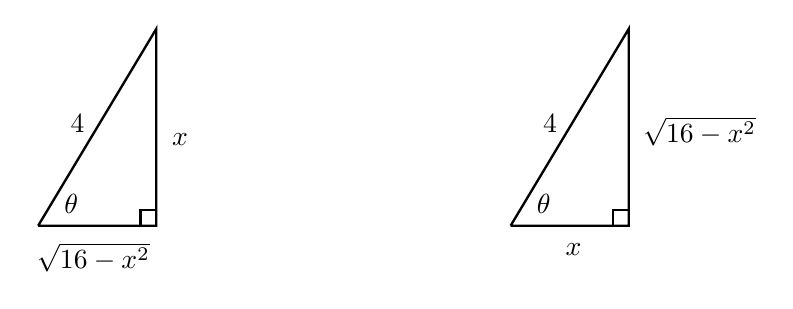
\begin{tikzpicture}
	\draw[line width=0.03cm] (0,0) -- (1.5,0) -- (1.5,2.5) -- (0,0);
	\draw[line width=0.03cm] (1.3,0) -- (1.3,0.2) -- (1.5,0.2);
	\node at (1.8,1.1) {$x$};
	\node at (0.7,-0.4) {$\sqrt{16 - x^2}$};
	\node at (0.5,1.3) {$4$};
	\node at (0.42,0.28) {$\theta$};
	
	\tikzset{shift={(6,0)}};

	\draw[line width=0.03cm] (0,0) -- (1.5,0) -- (1.5,2.5) -- (0,0);
	\draw[line width=0.03cm] (1.3,0) -- (1.3,0.2) -- (1.5,0.2);
	\node at (0.8,-0.3) {$x$};
	\node at (2.3,1.2) {$\;\;\sqrt{16 - x^2}$};
	\node at (0.5,1.3) {$4$};
	\node at (0.42,0.28) {$\theta$};
	\end{tikzpicture}
	\]
Using the right triangle on the left, we have $\sin \theta= \frac{x}{4}$, so that $x= 4 \sin \theta$ and $dx= 4 \cos \theta \;d\theta$. We also have $\cos \theta= \frac{\sqrt{16 - x^2}}{4}$, so that $\sqrt{16 - x^2}= 4 \cos \theta$. But then $(16 - x^2){1/2}= 4 \cos \theta$, which implies $(16 - x^2)^{3/2}= 4^3 \cos^3 \theta$. Therefore, we have\dots
	\[
	\int \dfrac{dx}{(16 - x^2)^{3/2}}= \int \dfrac{4 \cos \theta}{4^3 \cos^3 \theta} \;d\theta= \dfrac{1}{4^2} \int \dfrac{1}{\cos^2 \theta} \;d\theta= \dfrac{1}{16} \int \sec^2 \theta \;d\theta= \dfrac{1}{16} \,\tan \theta + C
	\]
But from the triangle, we know that $\tan \theta= \frac{x}{\sqrt{16 - x^2}}$. Therefore, we have\dots
	\[
	\int \dfrac{dx}{(16 - x^2)^{3/2}}= \boxed{\dfrac{x}{16 \sqrt{16 - x^2}} + C}
	\]
Alternatively, using the right triangle on the right above, we have $\cos \theta= \frac{x}{4}$, so that $x= 4 \cos \theta$ and $dx= -4 \sin \theta \;d\theta$. We also have $\sin \theta= \frac{\sqrt{16 - x^2}}{4}$, so that $\sqrt{16 - x^2}= 4 \sin \theta$. But then $(16 - x^2)^{1/2}= 4 \sin \theta$, which implies $(16 - x^2)^{3/2}= 4^3 \sin^3 \theta$. Therefore, we have\dots
	\[
	\hspace{-1.5cm} \int \dfrac{dx}{(16 - x^2)^{3/2}}= \int \dfrac{-4 \sin \theta}{4^3 \sin^3 \theta} \;d\theta= -\dfrac{1}{4^2} \int \dfrac{1}{\sin^2 \theta} \;d\theta= -\dfrac{1}{16} \int \csc^2 \theta \;d\theta= -\dfrac{1}{16} \cdot -\cot \theta + C= \dfrac{1}{16} \,\cot \theta + C
	\]
But from the triangle, we know that $\cot \theta= \frac{x}{\sqrt{16 - x^2}}$. Therefore, we have\dots
	\[
	\int \dfrac{dx}{(16 - x^2)^{3/2}}= \boxed{\dfrac{x}{16 \sqrt{16 - x^2}} + C}
	\]
}



% Question 5
\newpage
\question[10] {\itshape ``These integrals!'' cried Santa. ``These problems must be rigged.'' \par\phantom{(XX.. point)} ``No one reminded me, I had to be good at trig!} \par\vspace{0.3cm}

Showing all your work, compute the following:
	\[
	\int \sec^7 (\theta) \tan(\theta) \;d\theta
	\] \pspace

\vsol{\itshape We treat this as a trigonometric integral. If we choose $u= \tan \theta$, then $du= \sec^2 \theta \;d\theta$. Making this substitution, we would have $\sec^5 \theta$ term left in the integrand after `canceling' two of them from the $du$ term. But we can only replace even powers of secant from the Pythagorean identities. So, we instead choose $u= \sec \theta$. This implies that $du= \sec \theta \tan \theta \;d\theta$. But then\dots
	\[
	\begin{aligned}
	\int \sec^7 (\theta) \tan(\theta) \;d\theta=& \int \sec^6 \theta \cdot \sec \theta \tan \theta \;d\theta \\[0.3cm]
	&= \int u^6 \;du \\[0.3cm]
	&= \dfrac{u^7}{7} + C \\[0.3cm]
	&= \boxed{\dfrac{\sec^7 \theta}{7} + C}
	\end{aligned}
	\]
}



% Question 6
\newpage
\question[10] {\itshape All through the night, ole Santa worked---pressing on with cheer. \par\phantom{(XX.. point)} Suddenly, Santa froze and gasped. He'd forgotten his series this year!} \par\vspace{0.3cm}

Showing all your work and completely justifying your logic, determine whether the following series converges or diverges:
	\[
	\sum_{n=3}^\infty (-1)^n \,\dfrac{\ln n}{n}
	\] \pspace

\vsol{\small\itshape Because $\dfrac{\ln n}{n} \geq 0$ for $n \geq 3$ (because $\ln n, n \geq 0$ for these $n$), the given series alternates. We then try to apply the Alternating Series Test. 
	\begin{itemize}
	\item The sequence $\left\{ \dfrac{\ln n}{n} \right\}$ decreases: Observe that\dots
		\[
		\dfrac{d}{dn} \left( \dfrac{\ln n}{n} \right)= \dfrac{\frac{1}{n} \cdot n- 1 \cdot \ln n}{n^2}= \dfrac{1 - \ln n}{n^2}
		\]
	We know that $\ln n > 1$ for $n > e \approx 2.71828$. So, $1 - \ln n < 0$ for $n \geq 3$. Therefore, $\frac{d}{dn} \left( \frac{\ln n}{n} \right) < 0$ for $n \geq 3$, which proves that the sequence is decreasing. Alternatively, let $a_n= \frac{\ln n}{n}$. To show the sequence is decreasing, we need to show that $a_{n+1} < a_n$. We know that $\ds\lim_{n \to \infty} \left(1 + \frac{1}{n} \right)^n= e$ and that $\left(1 + \frac{1}{n} \right)^n$ increases with each $n$. But then if $n \geq 3$, we know that $\left(1 + \frac{1}{n} \right)^n < n$ for $n \geq 3$. But then using the fact that $\ln n$ is an increasing function, we have\dots
		\[
		\begin{gathered}
		\left(1 + \tfrac{1}{n} \right)^n < n \\
		\left( \tfrac{n + 1}{n} \right)^n < n \\
		\frac{(n + 1)^n}{n^n} < n \\
		(n + 1)^n < n^{n+1} \\
		\ln\left( (n + 1)^n \right) < \ln(n^{n+1}) \\
		n \ln(n+ 1) < (n+ 1) \ln n \\
		\dfrac{\ln(n+1)}{n+1} < \dfrac{\ln n}{n} \\
		a_{n+1} < a_n
		\end{gathered}
		\]
	
	\item $\ds\lim_{n \to \infty} \dfrac{\ln n}{n}= 0$: We can easily show this with lH\^opital's:
		\[
		\lim_{n \to \infty} \dfrac{\ln n}{n} \stackrel{\text{L.H.}}{=} \lim_{n \to \infty} \dfrac{\;\;\frac{1}{n}\;\;}{1}= \lim_{n \to \infty} \dfrac{1}{n}= 0
		\]
	\end{itemize}
Therefore, the series $\ds\sum_{n=3}^\infty (-1)^n \dfrac{\ln n}{n}$ converges by the Alternating Series Test.
	\[
	\boxed{\sum_{n=3}^\infty (-1)^n\, \dfrac{\ln n}{n} \text{ converges by A.S.T.}}
	\]
}



% Question 7
\newpage
\question[10] {\itshape What Santa knew about series wasn't quite true. \par\phantom{(XX.. point)} Turns out, he's gonna need some help getting through!} \par\vspace{0.3cm}

Showing all your work and completely justifying your logic, determine whether the following series converges or diverges:
	\[
	\sum_{n=0}^\infty \dfrac{(n!)^2}{(2n)!}
	\] \pspace

\vsol{\itshape Because of the factorial terms, we use the Ratio Test:
	\[
	\begin{aligned}
	\lim_{n \to \infty} \left| \dfrac{\;\;\dfrac{\big((n+1)! \big)^2}{\big(2(n+1)\big)!}}{\dfrac{(n!)^2}{(2n)!}} \right| &= \lim_{n \to \infty} \dfrac{\big((n+1)! \big)^2}{\big(2(n+1)\big)!} \cdot \dfrac{(2n)!}{(n!)^2} \\
	&= \lim_{n \to \infty} \dfrac{\big((n+1)! \big)^2}{(n!)^2} \cdot \dfrac{(2n)!}{\big(2(n+1)\big)!} \\[0.3cm]
	&= \lim_{n \to \infty} \dfrac{(n+1)! \cdot (n+1)!}{n! \cdot n!} \cdot \dfrac{(2n)!}{(2n + 2)!} \\[0.3cm]
	&= \lim_{n \to \infty} \dfrac{(n+1) \cdot n! \cdot (n + 1) \cdot n!}{n! \cdot n!} \cdot \dfrac{(2n)!}{(2n + 2)(2n + 1) (2n)!} \\[0.3cm]
	&= \lim_{n \to \infty} (n+1)(n+1) \cdot \dfrac{1}{(2n + 2)(2n +1)} \\[0.3cm]
	&= \lim_{n \to \infty} \dfrac{(n + 1)(n + 1)}{(2n + 2)(2n + 1)} \\[0.3cm]
	&= \lim_{n \to \infty} \dfrac{n^2 + 2n + 1}{4n^2 + 6n + 2} \\[0.3cm]
	&= \dfrac{1}{4} < 1
	\end{aligned}
	\]
Because this limit is less than 1, the series $\ds\sum_{n=0}^\infty \dfrac{(n!)^2}{(2n)!}$ is absolutely convergent by the Ratio Test. \par\vspace{0.1cm}
	\[
	\boxed{\sum_{n=0}^\infty \dfrac{(n!)^2}{(2n)!} \text{ converges absolutely}}
	\] \vfill
{\footnotesize Note. There are many better ways to compute the limit above.}
}



% Question 8
\newpage
\question[10] {\itshape Though the elves did their best, their calculations gave Santa a fright, \par\phantom{(XX.. point)} He ho'd, ``Bring help---these series might ground us tonight!''} \par\vspace{0.3cm}

Showing all your work and completely justifying your logic, determine whether the following series diverges, converges conditionally, or converges absolutely. 
	\[
	\sum_{n=0}^\infty \dfrac{(-1)^{n-1}}{7 + 2n}
	\] \par\vspace{0.1cm}

\vsol{\itshape Observe that $\frac{1}{7 + 2n}$ is positive for $n \geq 0$. Therefore, the given series is an Alternating Series. We test for convergence:
	\begin{itemize}
	\item The sequence $\left\{ \frac{1}{7 + 2n} \right\}$ is decreasing: Observe that $\frac{d}{dn} \left( \frac{1}{7 + 2n} \right)= -1(7 + 2n)^{-2} \cdot 2= \frac{-2}{(7 + 2n)^2}$, which is obviously negative for $n \geq 0$. Therefore, the sequence is decreasing. Alternatively, defining $a_n= \frac{1}{7 + 2n}$, we want to show $a_{n+1} < a_n$ in order to show $\{ a_n \}$ is decreasing. Observe\dots
		\[
		\begin{gathered}
		9 + 2n > 7 + 2n \\
		7 + 2 + 2n > 7 + 2n \\
		7 + 2(n + 1) > 7 + 2n \\
		\dfrac{1}{7 + 2(n + 1)} < \dfrac{1}{7 + 2n} \\
		a_{n+1} < a_n
		\end{gathered}
		\]
	Therefore, the sequence is decreasing. 
	
	\item $\ds\lim_{n \to \infty} \dfrac{1}{7 + 2n}= 0$: This limit is self-evident. 
	\end{itemize}
Therefore, the series $\ds\sum_{n=0}^\infty \dfrac{(-1)^{n-1}}{7 + 2n}$ converges by the Alternating Series Test. \pspace

To determine whether the series is absolutely or conditionally convergent, we need to determine whether the series $\ds\sum_{n=0}^\infty \dfrac{1}{7 + 2n}$ diverges or converges. Observe that\dots
	\[
	\sum_{n=0}^\infty \dfrac{1}{7 + 2n} > \sum_{n=0}^\infty \dfrac{1}{7n + 9 + 2n}= \sum_{n=0}^\infty \dfrac{1}{9n + 9}= \dfrac{1}{9} \sum_{n=0}^\infty \dfrac{1}{n + 1}= \dfrac{1}{9} \sum_{n=1}^\infty \dfrac{1}{n}
	\]
The series $\ds\sum_{n=1}^\infty \dfrac{1}{n}$ diverges by the $p$-test with $p= 1$, or because it is the well-known Harmonic Series---which diverges. Therefore, $\ds\sum_{n=0}^\infty \dfrac{1}{7 + 2n}$ diverges by the Direct Comparison Test.}

\vsol{%
\newpage
{
\thispagestyle{empty}
Alternatively, we know that $\ds\sum_{n=1}^\infty \dfrac{1}{n}$ diverges by the reasoning we just mentioned. Now we have\dots
	\[
	\lim_{n \to \infty} \dfrac{\;\;\dfrac{1}{7 + 2n}\;\;}{\dfrac{1}{n}}= \lim_{n \to \infty} \dfrac{n}{7 + 2n}= \dfrac{1}{2} < \infty
	\]
and this limit is not zero. Therefore, by the Limit Comparison Test, we know that $\ds\sum_{n=0}^\infty \dfrac{1}{7 + 2n}$ and $\ds\sum_{n=1}^\infty \dfrac{1}{n}$ have the same type of convergence. Therefore, $\ds\sum_{n=0}^\infty \dfrac{1}{7 + 2n}$ diverges. \pspace

Alternatively, let $f(x)= \frac{1}{7 + 2x}$. It is clear that $f(x)$ is continuous for all $x \neq -\frac{7}{2}$. The same work above shows that $f(x)$ is positive and decreasing. But then by the Integral Test, we know that $\ds\sum_{n=0}^\infty \dfrac{1}{7 + 2n}$ converges if and only if $\ds\int_0^\infty f(x) \;dx$ converges. Observe that\dots
	\[
	\int_0^\infty \dfrac{dx}{7 + 2x}:= \lim_{b \to \infty} \int_0^b \dfrac{dx}{7 + 2x}= \lim_{b \to \infty} \frac{1}{2}\,\ln|7 + 2x| \bigg|_0^b= \lim_{b \to \infty} \dfrac{1}{2} \ln|7 + 2b| - \dfrac{1}{2}\,\ln|7|= \infty
	\]
But then the series $\ds\sum_{n=0}^\infty \dfrac{1}{7 + 2n}$ diverges. \pspace

Because the series $\ds\sum_{n=0}^\infty \dfrac{(-1)^{n-1}}{7 + 2n}$ converges but the series $\ds\sum_{n=0}^\infty \dfrac{1}{7 + 2n}$ diverges, the series $\ds\sum_{n=0}^\infty \dfrac{(-1)^{n-1}}{7 + 2n}$ converges conditionally. 
	\[
	\boxed{\sum_{n=0}^\infty \dfrac{(-1)^{n-1}}{7 + 2n} \text{ converges conditionally}}
	\]
\setcounter{page}{10}
}
}



% Question 9
\newpage
\question[10] {\itshape Santa's trajectory not correct, ``Someone help me!'' \par\phantom{(XX.. point)} No one told me I that couldn't use Chat-GPT!} \par\vspace{0.3cm}

Showing all your work and completely justifying your logic, determine whether the series below converges or diverges. If the series converges, find its sum. If it diverges, explain why.
	\[
	\sum_{n=0}^\infty \dfrac{3}{2^{n-1}}
	\] \pspace

\vsol{\itshape We first rewrite the summand:
	\[
	\sum_{n=0}^\infty \dfrac{3}{2^{n-1}}= \sum_{n=0}^\infty \dfrac{3}{2^n \cdot 2^{-1}}= \sum_{n=0}^\infty \dfrac{6}{2^n}= \sum_{n=0}^\infty 6 \cdot \dfrac{1}{2^n}= \sum_{n=0}^\infty 6 \left( \dfrac{1}{2} \right)^n
	\]
Because this series has the form $\ds\sum_n^\infty a r^n$, this series is geometric with $a= 6$ and $r= \frac{1}{2}$. Because $|r|= \frac{1}{2} < 1$, we know that the series converges by the Geometric Series Test. Furthermore, we know that the series converges to\dots
	\[
	\sum_{n=0}^\infty \dfrac{3}{2^{n-1}}= \frac{\text{first term}}{1 - r}= \dfrac{6 \cdot 1}{1 - \frac{1}{2}}= \dfrac{\;\;6\;\;}{\frac{1}{2}}= 12
	\] \pspace
Therefore,
	\[
	\boxed{\sum_{n=0}^\infty \dfrac{3}{2^{n-1}}= 12}
	\]
}



% Question 10
\newpage
\question[10] {\itshape Santa hurtled through the sky, the fate of Christmas so near, \par\phantom{(XX.. point)} But he shook with fear, the series were too tricky to handle this year!} \par\vspace{0.3cm}

Showing all your work and completely justifying your logic, determine whether the following series converges or diverges:
	\[
	\sum_{n=1}^\infty \dfrac{5n}{n^3 + 4}
	\] \pspace

\vsol{\itshape For `large' $n$, the numerator `looks like' $n$ while the denominator `looks like' $n^3$, so the whole fraction `looks like' $\frac{n}{n^3}= \frac{1}{n^2}$. We know that the series $\sum \frac{1}{n^2}$ converges. So, we predict that this series converges. We can prove this using the Limit Comparison Test:
	\[
	\lim_{n \to \infty} \dfrac{\;\;\dfrac{5n}{n^3 + 4}\;\;}{\dfrac{1}{n^2}}= \lim_{n \to \infty} \dfrac{5n^3}{n^3 + 4}= 5 < \infty
	\]
Because this limit is finite and nonzero, we know from the Limit Comparison Test that $\ds\sum_{n=1}^\infty \dfrac{5n}{n^3 + 4}$ and $\ds\sum_{n=1}^\infty \dfrac{1}{n^2}$ have the same behavior. Because the series $\ds\sum_{n=1}^\infty \dfrac{1}{n^2}$ converges by the $p$-test (in fact, it converges to $\frac{\pi^2}{6}$), it must be that the series $\ds\sum_{n=1}^\infty \dfrac{5n}{n^3 + 4}$ converges. 
	\[
	\boxed{\sum_{n=1}^\infty \dfrac{5n}{n^3 + 4} \text{ Converges}}
	\] \pspace
Alternatively, we can use the Direct Comparison Test. Observe that\dots
	\[
	\sum_{n=1}^\infty \dfrac{5n}{n^3 + 4} < \sum_{n=1}^\infty \dfrac{5n}{n^3}= 5 \sum_{n=1}^\infty \dfrac{1}{n^2}
	\]
Because the series $\ds\sum_{n=1}^\infty \dfrac{1}{n^2}$ converges by the $p$-test (in fact, it converges to $\frac{\pi^2}{6}$), it must be that the series $\ds\sum_{n=1}^\infty \dfrac{5n}{n^3 + 4}$ converges by the Direct Comparison Test.
	\[
	\boxed{\sum_{n=1}^\infty \dfrac{5n}{n^3 + 4} \text{ Converges}}
	\] 
}



% Question 11
\newpage
\question[10] {\itshape Santa puzzled through power series, each term driving him insane, \par\phantom{(XX.. point)} But ``At this rate, I’m as safe as a budget Boeing plane!''} \par\vspace{0.3cm}

Showing all your work and completely justifying your logic, determine the center, radius, and interval of convergence for the following power series:
	\[
	\sum_{n=0}^\infty (-1)^n \, \dfrac{(x + 6)^n}{n!}
	\] \pspace

\vsol{\itshape Observe that $x= -6$ makes the summand 0. Therefore, $x= -6$ is the center of the series. We can use the Ratio Test to find a criterion for convergence:
	\[
	\begin{aligned}
	\lim_{n \to \infty} \left| \dfrac{\;\;(-1)\, \dfrac{(x + 6)^{n+1}}{(n + 1)!}\;\;}{(-1)^n\, \dfrac{(x + 6)^n}{n!}} \right|&= \lim_{n \to \infty} \left| \dfrac{(x + 6)^{n+1}}{(n + 1)!} \cdot \dfrac{n!}{(x + 6)^n} \right| \\
	&= \lim_{n \to \infty} \left| \dfrac{(x + 6)^{n+1}}{(x + 6)^n} \cdot \dfrac{n!}{(n + 1)!} \right| \\
	&= \lim_{n \to \infty} \left| (x + 6) \cdot \dfrac{n!}{(n + 1)n!} \right| \\
	&= \lim_{n \to \infty} \left| \dfrac{x + 6}{n + 1} \right| \\
	&= 0 < 1
	\end{aligned}
	\]
Observe that this limit is less than 1 for all $x$. Therefore, the Ratio Test states that the series is absolutely convergent for all real numbers $x$. Therefore, the radius of convergence is infinite and the interval of convergence is $\mathbb{R}$, i.e. all real numbers. \pspace
	\[
	\boxed{%
	\begin{gathered}
	\text{Center: } x= -6 \\
	R= \infty \\
	\text{Interval Convergence: } (-\infty, \infty)
	\end{gathered}}
	\]
}



% Question 12
\newpage
\question[10] {\itshape As he plotted his course, Santa frowned at each point of divergence,, \par\phantom{(XX.. point)} For he couldn’t take flight till someone helped find his interval of convergence.} \par\vspace{0.3cm}

Showing all your work and completely justifying your logic, determine the center, radius, and interval of convergence for the following power series:
	\[
	\sum_{n=1}^\infty \dfrac{x^n}{n\, 3^n}
	\] \pspace

\vsol{\small\itshape Observe that $x= 0$ makes the summand 0. Therefore, $x= 0$ is the center of the series. We can use the Ratio Test to find a criterion for convergence:
	\[
	\hspace{-2.5cm} \lim_{n \to \infty} \left| \dfrac{\;\;\dfrac{x^{n+1}}{(n+1) 3^{n+1}}\;\;}{\dfrac{x^n}{n\,3^n}} \right|= \lim_{n \to \infty} \left| \dfrac{x^{n+1}}{(n+1) 3^{n+1}} \cdot \dfrac{n\, 3^n}{x^n} \right| 
	= \lim_{n \to \infty} \left| \dfrac{x^{n+1}}{x^n} \cdot \dfrac{3^n}{3^{n+1}} \cdot \dfrac{n}{n+1} \right| 
	= \lim_{n \to \infty} \left| x \cdot \dfrac{1}{3} \cdot \dfrac{n}{n+ 1} \right| 
	= \left| x \cdot \dfrac{1}{3} \cdot 1 \right| 
	= \left| \dfrac{x}{3} \right|
	\]
Alternatively, we could use the Root Test:
	\[
	\lim_{n \to \infty} \left| \dfrac{x^n}{n \,3^n} \right|^{1/n}= \lim_{n \to \infty} \left| \dfrac{x}{\sqrt[n]{n} \, 3} \right|= \left| \dfrac{x}{1 \cdot 3} \right|= \left| \dfrac{x}{3} \right|
	\]
For either of these tests to guaranteed convergence, we need\dots
	\[
	\begin{gathered}
	\left| \dfrac{x}{3} \right| < 1 \\
	-1 < \dfrac{x}{3} < 1 \\
	-3 < x < 3
	\end{gathered}
	\]
This implies that the radius of convergence is $R= \frac{3 - (-3)}{2}= \frac{6}{2}= 3$. We need now test the endpoints: \pspace

$x= -3$: If $x= -3$, we have the series $\ds\sum_{n=1}^\infty \dfrac{(-3)^n}{n\, 3^n}= \sum_{n=1}^\infty \dfrac{(-1)^n 3^n}{n\, 3^n}= \sum_{n=1}^\infty \dfrac{(-1)^n}{n}$, which is an alternating series. Observe that the sequence $\left\{ \frac{1}{n} \right\}$ is decreasing and $\ds\lim_{n \to \infty} \frac{1}{n}= 0$. Therefore, the series $\ds\sum_{n=1}^\infty \dfrac{(-1)^n}{n}$ converges by the Alternating Series Test. Alternatively, we recognize this as the Alternating Harmonic Series, which we know converges to $\ln(2)$. \pspace

$x= 3$: If $x= 3$, we have the series $\ds\sum_{n=1}^\infty \dfrac{3^n}{n\, 3^n}= \sum_{n=1}^\infty \dfrac{1}{n}$. This series diverges by the $p$-test with $p= 1$. Alternatively, we recognize this as the Harmonic series, which diverges. 

Because the series converges at $x= -3$ and for $x \in (-3, 3)$ but diverges at $x= 3$, the interval of convergence is $[-3, 3)$. 
	\[
	\boxed{%
	\begin{gathered}
	\text{Center: } x= 0 \\
	R= 3 \\
	\text{Interval Convergence: } [-3, 3)
	\end{gathered}}
	\]
}



% Question 13
\newpage
\question[10] {\itshape As he tallied the sum, Santa muttered, ``These terms never cease!'' \par\phantom{(XX.. point)} ``If this series keeps growing, I’ll be stuck here till after next Christmas feast!''} \par\vspace{0.3cm}
	\begin{enumerate}[(a)]
	\item Use the Maclaurin series for $\cos(x)$ to find a Maclaurin series for $x \cos(x^2)$. \pspace
	
		\psol{\itshape We know that $\ds\cos x= \sum_{n=0}^\infty (-1)^n\, \dfrac{x^{2n}}{(2n)!}$ and is valid for all $x$. But then\dots}
			\[
			\begin{aligned}
			\psol{\cos x= \sum_{n=0}^\infty (-1)^n\, \dfrac{x^{2n}}{(2n)!}} \phantom{==========.} \\[0.2cm]
			\psol{\cos(x^2)= \sum_{n=0}^\infty (-1)^n\, \dfrac{(x^2)^{2n}}{(2n)!}= \sum_{n=0}^\infty (-1)^n\, \dfrac{x^{4n}}{(2n)!}} \\[0.2cm]
			\psol{x \cos(x^2)= x \sum_{n=0}^\infty (-1)^n\, \dfrac{x^{4n}}{(2n)!}= \boxed{\sum_{n=0}^\infty (-1)^n\, \dfrac{x^{4n + 1}}{(2n)!}}}
			\end{aligned}
			\]
		\par\vspace{1.7cm}
	
	\item Use (a) to compute the following sum:
		\[
		\sum_{n=0}^\infty (-1)^n \, \dfrac{\pi^{\frac{4n+1}{2}}}{(2n)!}
		\] \pspace
	
	\vsol{\itshape We know from the previous part that $\ds x \cos(x^2)= \sum_{n=0}^\infty (-1)^n\, \dfrac{x^{4n + 1}}{(2n)!}$ and that this is valid for all $x$. But then\dots
			\[
			\begin{aligned}
			\sum_{n=0}^\infty (-1)^n \, \dfrac{\pi^{\frac{4n+1}{2}}}{(2n)!}&= \sum_{n=0}^\infty (-1)^n \, \dfrac{\pi^{\frac{1}{2}\,(4n + 1)}}{(2n)!} \\[0.2cm]
			&= \sum_{n=0}^\infty (-1)^n \, \dfrac{(\sqrt{\pi})^{4n+1}}{(2n)!} \\[0.2cm]
			&= \sqrt{\pi} \cos\big( (\sqrt{\pi})^2) \\[0.2cm]
			&= \sqrt{\pi} \cos(\pi) \\[0.2cm]
			&= \sqrt{\pi} \cdot -1 \\[0.2cm]
			&= \boxed{-\sqrt{\pi}}
			\end{aligned}
			\]
		}
	\end{enumerate}



% Question 14
\newpage
\question[10] {\itshape Five golden rings, four calling birds, three French hens, \par\phantom{(XX.. points)} Two turtle doves, and a partridge in a pear tree! \par\phantom{(XX.. points)} \dots but they were all of them deceived for another ring was made.} \par\vspace{0.3cm}

Define the function $f(x)$ to be $f(x)= x e^{-x^4}$. 
        \begin{enumerate}[(a)]
        \item Using a known power series, express $f(x)$ as an infinite series. \pspace
        
	        \psol{\itshape We know that the Maclaurin series for $e^x$ is $\ds\sum_{n=0}^\infty \dfrac{x^n}{n!}$ and is valid for all $x$. But then\dots}
			\[
			\begin{aligned}
			\psol{e^x= \sum_{n=0}^\infty \dfrac{x^n}{n!}} \phantom{=============....} \\[0.2cm]
			\psol{e^{-x^4}= \sum_{n=0}^\infty \dfrac{(-x^4)^n}{n!}= \sum_{n=0}^\infty (-1)^n\,\dfrac{x^{4n}}{n!}} \phantom{==..} \\[0.2cm]
			\psol{xe^{-x^4}= x \sum_{n=0}^\infty (-1)^n\, \dfrac{x^{4n}}{n!}= \boxed{\sum_{n=0}^\infty (-1)^n\,\dfrac{x^{4n + 1}}{n!}}}
			\end{aligned}
			\] \par\vspace{1.2cm}

        \item Use your answer from (a) to express the following integral as a series:
	        	\[
        		\int x e^{-x^4} \;dx
	        	\] \pspace
		
		\vsol{\itshape We have\dots
			\[
			\begin{aligned}
			\int x e^{-x^4} \;dx&= \int \sum_{n=0}^\infty (-1)^n\,\dfrac{x^{4n + 1}}{n!} \;dx \\[0.3cm]
			&= \sum_{n=0}^\infty \int (-1)^n\,\dfrac{x^{4n + 1}}{n!} \;dx \\[0.3cm]
			&= \sum_{n=0}^\infty \dfrac{(-1)^n}{n!} \int x^{4n+1} \;dx \\[0.3cm]
			&= \boxed{C + \sum_{n=0}^\infty \dfrac{(-1)^n x^{4n + 2}}{n! (4n + 2)}} 
			\end{aligned}
			\]
		}
        \end{enumerate}



% Question 15
\newpage
\question[10] {\itshape With presents delivered and Christmas nearly in the clear, \par\phantom{(XX.. point)} Santa has one last task, and then you're done for this year!} \par\vspace{0.3cm}

Showing all your work, find the third degree Taylor polynomial, $T_3(x)$, centered at $x= 0$ for the function $f(x)= \sqrt{x + 1}$. \pspace

\vsol{\itshape We know that the Taylor series of degree $N$ centered at $x= a$ is given by $\ds T_N(x)= \sum_{n=0}^N \dfrac{f^{(n)}(a)}{n!} \, (x - a)^n$. We have $a= 0$ and $f(x)= \sqrt{x + 1}$. So, we need only compute the value of the derivatives up to order $N= 3$:
	\[
	\begin{aligned}
	f(x)&= \sqrt{x + 1} \bigg|_{x=0}= \sqrt{1}= 1 \\[0.3cm]
	f'(x)&= \dfrac{d}{dx}\, (x + 1)^{1/2}= \dfrac{1}{2 \sqrt{x + 1}} \bigg|_{x=0}= \dfrac{1}{2 \sqrt{1}}= \dfrac{1}{2} \\[0.3cm]
	f''(x)&= \dfrac{d}{dx}\, \dfrac{1}{2}\, (x + 1)^{-1/2}= -\dfrac{1}{4 (x + 1)^{3/2}} \bigg|_{x=0}= -\dfrac{1}{4 (1)}= -\dfrac{1}{4} \\[0.3cm]
	f'''(x)&= \dfrac{d}{dx}\, -\dfrac{1}{4} (x + 1)^{3/2}= \dfrac{3}{8 (x + 1)^{5/2}}= \dfrac{3}{8(1)}= \dfrac{3}{8} 
	\end{aligned}
	\] \par\vspace{0.3cm}
But then the third degree Taylor polynomial is given by\dots
	\[
	\begin{aligned}
	T_3(x)&= \sum_{n=0}^3 \dfrac{f^{(n)}(a)}{n!} \, (x - a)^n \\[0.3cm]
	&= \dfrac{f(0)}{0!} \,(x - 0)^0 + \dfrac{f'(0)}{1!}\, (x - 0)^1 + \dfrac{f''(0)}{2!}\, (x - 0)^2 + \dfrac{f'''(0)}{3!}\, (x - 0)^3 \\[0.3cm]
	&= f(0) + f'(0) \,x + \dfrac{f''(0)}{2}\, x^2 + \dfrac{f'''(0)}{6}\, x^3 \\[0.3cm]
	&= 1 + \dfrac{x}{2} + \dfrac{-1/4}{2}\, x^2 + \dfrac{3/8}{6}\, x^3 \\[0.3cm]
	&= \boxed{1 + \dfrac{x}{2} - \dfrac{x^2}{8} + \dfrac{x^3}{16}}
	\end{aligned}
	\]
}
\end{questions}

% End Poem
\newpage

\phantom{.} \vfill
	\begin{table}[h]
	\centering
	\begin{tabular}{l}
	{\itshape The night was set right and magic of Christmas came true.} \\
	{\itshape Santa let out a sigh, these students really came through.} \\
	{\itshape Each integral untangled, each convergence made precise,} \\
	{\itshape They restored all the magic that keeps Christmas nice.} \\
	\\
	{\itshape And Santa called out as he rode through the night,} \\
	{\itshape His voice full of cheer and his heart lifted light:} \\
	{\itshape ``Merry Christmas to all! But before I depart,} \\
	{\itshape Never forget your Calculus---the math of the heart!''} 
	\end{tabular}
	\end{table}
\phantom{.} \vfill

\end{document}